\documentclass[acmtog, review, anonymous]{acmart}

\usepackage{booktabs} % For formal tables
\usepackage{multirow}
\usepackage{wrapfig}

\usepackage{makecell}

\renewcommand\theadalign{bc}
\renewcommand\theadfont{\bfseries}
\renewcommand\theadgape{\Gape[4pt]}
\renewcommand\cellgape{\Gape[4pt]}

% TOG prefers author-name bib system with square brackets
\citestyle{acmauthoryear}
\setcitestyle{square}


\usepackage[ruled, linesnumbered]{algorithm2e} % For algorithms
\renewcommand{\algorithmcfname}{ALGORITHM}
\SetAlFnt{\small}
\SetAlCapFnt{\small}
\SetAlCapNameFnt{\small}
\SetAlCapHSkip{0pt}
\IncMargin{-\parindent}
\SetKwRepeat{Do}{do}{while}

\usepackage{amsmath}
\DeclareMathOperator*{\argmax}{argmax}
\DeclareMathOperator*{\argmin}{argmin}

% strike out old text for revision
\usepackage[normalem]{ulem}
 
% Metadata Information
\acmJournal{TOG}
% \acmVolume{9}
% \acmNumber{4}
% \acmArticle{39} 
% \acmYear{2010}
% \acmMonth{3}

% Copyright
%\setcopyright{acmcopyright}
%\setcopyright{acmlicensed}
%\setcopyright{rightsretained}
%\setcopyright{usgov}
% \setcopyright{usgovmixed} 
%\setcopyright{cagov}
%\setcopyright{cagovmixed}

% DOI
% \acmDOI{0000001.0000001_2}

% Paper history
% \received{February 2007}
% \received{March 2009}
% \received[final version]{June 2009}
% \received[accepted]{July 2009}

% Document starts
\begin{document}
% Title portion
%\title{OptCuts: Joint Cutting and Parameterization of 3D Surfaces} 
\title{OptCuts: Joint Optimization of Surface Cuts and Parameterization
\\ {\small (Paper ID: 243)}
} 

\author{Minchen Li}
% \orcid{1234-5678-9012-3456}
% \affiliation{%
%   \institution{College of William and Mary}
%   \streetaddress{104 Jamestown Rd}
%   \city{Williamsburg}
%   \state{VA}
%   \postcode{23185}
%   \country{USA}}
\email{minchernl@gmail.com}
% \author{Valerie B\'eranger}
% \affiliation{%
%   \institution{Inria Paris-Rocquencourt}
%   \city{Rocquencourt}
%   \country{France}
% }
% \email{beranger@inria.fr}
% \author{Aparna Patel} 
% \affiliation{%
%  \institution{Rajiv Gandhi University}
%  \streetaddress{Rono-Hills}
%  \city{Doimukh} 
%  \state{Arunachal Pradesh}
%  \country{India}}
% \email{aprna_patel@rguhs.ac.in}
% \author{Huifen Chan}
% \affiliation{%
%   \institution{Tsinghua University}
%   \streetaddress{30 Shuangqing Rd}
%   \city{Haidian Qu} 
%   \state{Beijing Shi}
%   \country{China}
% }
% \email{chan0345@tsinghua.edu.cn}
% \author{Ting Yan}
% \affiliation{%
%   \institution{Eaton Innovation Center}
%   \city{Prague}
%   \country{Czech Republic}}
% \email{yanting02@gmail.com}
% \author{Tian He}
% \affiliation{%
%   \institution{University of Virginia}
%   \department{School of Engineering}
%   \city{Charlottesville}
%   \state{VA}
%   \postcode{22903}
%   \country{USA}
% }
% \affiliation{%
%   \institution{University of Minnesota}
%   \country{USA}}
% \email{tinghe@uva.edu}
% \author{Chengdu Huang}
% \author{John A. Stankovic}
% \author{Tarek F. Abdelzaher}
% \affiliation{%
%   \institution{University of Virginia}
%   \department{School of Engineering}
%   \city{Charlottesville}
%   \state{VA}
%   \postcode{22903}
%   \country{USA}
% }

\renewcommand\shortauthors{Li, M. et al}

\definecolor{gray}{rgb}{0.5,0.5,0.5}
\definecolor{green}{rgb}{0, 0.6, 0}
\definecolor{orange}{rgb}{1, 0.5, 0}
\definecolor{mahogany}{rgb}{0.75, 0.25, 0.0}
\definecolor{purple}{rgb}{0.6, 0.1, 0.6}
\definecolor{darkgreen}{rgb}{0, 0.3, 0}
\definecolor{orange}{rgb}{1, 0.5, 0.}
\newcommand{\minchen}[1]{\textcolor{blue}{\textbf{Minchen: #1}}}
\newcommand{\justin}[1]{\textcolor{red}{\textbf{Justin: #1}}}
\newcommand{\alla}[1]{\textcolor{orange}{\textbf{Alla: #1}}}
\newcommand{\danny}[1]{\textcolor{purple}{\textbf{Danny: #1}}}
\newcommand{\vova}[1]{\textcolor{green}{\textbf{Vova: #1}}}
% for revision:
\newcommand{\revised}[1]{\textcolor{red}{\textbf{#1}}}
\newcommand{\old}[1]{\textcolor{green}{\sout{#1}}}
% after revision finalized, use:
% \newcommand{\revised}[1]{{#1}}
% \newcommand{\old}[1]{} 

\begin{teaserfigure} 
\centering
  \vspace{-0.2cm}
  \includegraphics[width=\linewidth]{fig/teaser/teaser.pdf}
  \vspace{-0.6cm}
  \caption{Starting from an initial embedding (left), we show the iteration process of our OptCuts algorithm jointly optimizing surface cuts and mapping distortion while enforcing global bijectivity. OptCuts iteratively updates
  continuous changes in the embedding vertices, as well as discrete topological changes in the UV mesh by propagating simple and local topology splitting and merging operations. In this example the bound is set to $4.1$, measured using the symmetric Dirichlet distortion energy~\cite{Smith2015Bijective}, with total inner iterations reported at each rendered frame. }
  \label{fig:teaser}
\end{teaserfigure}

\begin{abstract}
% context and need
Low-distortion mapping of three-dimensional surfaces to the plane is a critical problem in geometry processing. The intrinsic distortion introduced by such UV mappings is highly dependent on the choice of surface cuts that form seamlines 
which break mapping continuity.
%across which the mapping is not continuous.  
%Most such surfaces require cutting and distortion to produce a valid map. 
%Existing techniques largely consider seam placement and distortion minimization independently, first placing seams and then minimizing distortion; this leads to suboptimal output. Some recent attempts to address this issue ask the user to choose a potentially counterintuitive parameter weighting between seam quality and distortion and can require manual intervention to obtain a quality result. 
%\vova{Above does not encapsulate geometry images and olga's greedy seaming approach. At the same time I don't want to over-crowd abstract with these details. 
%Maybe we skip the discussion of previous work here simply motivate our approach? ``A 3D artist typically aims at a UV map that does not exceed certain distortion level (which might lead to stretching artifacts), while minimizing the seam length (which lead to discontinuities). Motivated by this observation, we propose a novel problem formulation and a joint discrete continuous optimization method...''} As an alternative, 
Parameterization applications typically require UV maps with an application-specific upper bound on distortion to avoid mapping artifacts; at the same time they seek to reduce cut lengths to minimize discontinuity artifacts. 
%Motivated by these observations,
%
We propose {\em OptCuts}, an algorithm for jointly optimizing the parameterization and cutting of a three-dimensional mesh. 
%OptCuts automatically seeks to minimize seam lengths subject to satisfying a user-provided bound on the distortion of the mapping computed using these seams. 
%\alla{what does topology or geometry descent mean?}
%Starting with an arbitrary initial embedding, OptCuts alternates between discrete topology descent and smooth geometry descent to search for an optimal UV map strictly satisfying a specified distortion bound. 
OptCuts starts from an arbitrary initial embedding and a user-requested distortion bound. It requires no parameter setting and automatically seeks to minimize seam lengths subject to satisfying the distortion bound of the mapping computed using these seams.
%as such it can be used to improve pre-existing mappings or can start from scratch to build an entirely new embedding. Starting with an arbitrary initial embedding, 
OptCuts alternates between topology and geometry update steps that consistently decrease distortion and seam length, producing a UV map with compact boundaries that strictly satisfies the distortion bound. 
%OptCuts takes 
%Aside from this user-desired bound, OptCuts requires no further parameter setting. 
OptCuts automatically produces high-quality, globally bijective UV maps without user intervention. 
While OptCuts can thus be a highly effective tool to create new mappings from scratch, we also show how it can be employed to improve pre-existing embeddings.  Additionally, when semantic or other priors on seam placement are desired, OptCuts can be extended to respect these user preferences as constraints during optimization of the parameterization.
We demonstrate the scalable performance of OptCuts on a wide range of challenging benchmark parameterization examples, as well as in comparisons with state-of-the-art UV methods and commercial tools.   
%
%and can generate seams whose structure is informed by a range of standard distortion measures as well as user preferences on regional seam placement.
%We also demonstrate extensions in our optimization framework enabling global bijectivity and incorporating user guidance. 
%
%\vova{Removed: ``seamlessness, and other discrete-continuous geometry processing problems''. AFAIK we are not planning to show it, correct?}
\end{abstract}


%
% The code below should be generated by the tool at
% http://dl.acm.org/ccs.cfm
% Please copy and paste the code instead of the example below. 
%
\begin{CCSXML}
<ccs2012>
	<concept>
		<concept_id>10010147.10010371.10010396.10010398</concept_id>
		<concept_desc>Computing methodologies~Mesh geometry models</concept_desc>
		<concept_significance>500</concept_significance>
	</concept>
</ccs2012>
\end{CCSXML}

\ccsdesc[500]{Computing methodologies~Mesh geometry models}

%
% End generated code
%


\keywords{geometry processing, mesh parameterization, seam placement, numerical optimization}



\maketitle

% !TeX root = OptCuts.tex

\section{Introduction}
% context
Mapping three-dimensional meshes to the plane is a fundamental task in computer graphics.  The two-dimensional mesh embeddings produced by mapping methods are commonly used to store reflectance functions, normals, and displacements
for the mesh, providing a domain for painting, synthesizing, and manipulating texture and geometric details. 
%Mesh parameterization is a critical task in computer graphics, with applications including texture mapping, remeshing, and detail transfer.  
%\vova{I removed non-texture apps for now, because I'm not sure if our formulation is as easy to motivate for remeshing and detail transfer.}
%
The usability of these embeddings is highly dependent on two interconnected factors: the surface distortion introduced by the mapping and the length of the surface cuts, forming seams across which the mapping is discontinuous~\cite{Hormann2008}. Both high distortion and longer seams are detrimental to downstream applications. Yet, reducing distortion below a desired 
%some %intrinsic surface %<--- what does this mean
bound typically requires introducing longer seams. 
% To do so, parameterization tools must cope with intertwined challenges in topology and geometry:  a high-quality parameterization must cut a surface into simple %disk-shape 
%patches so that each can be mapped to the plane with a reasonably small level of distortion.

Given its broad applicability, parameterization has long been a focus of research in geometry processing. Algorithms in this domain focus on these two key aspects of the problem \cite{Sheffer07_ParameterizationSurvey}.  Particularly well-studied are \emph{geometric} techniques that assume a surface has already been cut into disk-topology segments %charts %<--- charts are the maps
 which each then need to be mapped into the plane with minimal distortion while maintaining fixed connectivity; at this point, parameterization becomes a real-valued optimization problem that seeks to minimize changes in mesh angles and areas while maintaining local or global injectivity. Complementing these techniques, \emph{topological} algorithms find reasonable seams, either keeping the surface in one piece or partitioning it into individual segments that can then be parameterized with low distortion. %(Section~\ref{sec:related}).   

In contrast, we propose a joint optimization algorithm {\em OptCuts} that simultaneously optimizes for both seam length and the corresponding distortion of the embedding.
Our algorithm is based on a minimization model problem that directly and automatically balances between seam length and parametric distortion measures. Manually balancing distortion and seam quality requires a choice of a relative scaling factor between these two objectives. From a practical perspective, it is difficult for users to choose this factor as the two terms measure very different quantities and no such setting can provide a guarantee on the quality of the generated map's distortion. 
On the other hand, users typically have a clear sense of the amount of distortion they consider acceptable for their application. Motivated by this observation we cast our coupled seam and distortion optimization as a \emph{constrained} problem to find charts with locally minimal seam lengths that strictly satisfy a user-set distortion bound. Treating the distortion bound as a hard inequality constraint guarantees a pre-specified level of mapping quality, while enabling us to explore optimal seams that satisfy this bound. %In turn, o %<--- not sure what ``in turn'' means in this context

Prior methods coupling distortion reduction and cutting have generally required hand-tuning a number of user-exposed parameters and, as in the recently proposed AutoCuts~\cite{Poranne2017Autocuts}, even advocate manual intervention by interactively adjusting these parameters during the optimization process.

In contrast, OptCuts is a fully automatic optimization method: users provide their desired distortion bound and OptCuts then directly computes a parametrization satisfying this bound with locally minimal edge lengths. Maps provided are always locally injective and, as we will show, can additionally be constrained to be bijective and even support additional, user-provided seam placement constraints and biases when desired. 
%Likewise, as 
As demonstrated by our comparisons in Section~\ref{sec:results},
%, e.g.\ Figure~\ref{fig:autocut} 
%and ???~\danny{update when all comparison figures and tables are in.}, 
when compared to previous methods that do provide an automatic mode~\cite{BoundedDistortParam:2002,Poranne2017Autocuts}, OptCuts produces much shorter seams when its bound is set for the same achieved distortion. 
%Even in comparing to hand-tuned UV maps, we find that OptCuts consistently finds similar seam lengths for comparable or even better distortion bounds; see e.g., Figures ??? \danny{update when all comparison figures and tables are in.}. 
Likewise, as we show in Section~\ref{sec:var}, e.g. Figure \ref{fig:comp_Seamster}, OptCuts can also be used to polish any preexisting UV map irrespective of the method used to create it. OptCuts can take an arbitrary UV map as input and improve either seam length while preserving the current distortion bound or even improve upon distortion as well, by setting a lower distortion bound.

  To achieve these gains we begin by casting global parameterization as a constrained minimization, formulated with seam length as our objective and a distortion bound as our inequality constraint. We then observe that the \emph{Lagrangian} of this constrained minimization's saddle-point problem directly captures a multi-objective optimization formed by the weighted sum of our seam length measure and map distortion. However, the key observation here is that now there is a natural scaling implied between the two measures that is directly defined by the Lagrange multiplier of the distortion bound. Regularization of iterated updates to this multiplier then allow us to smoothly explore variations of the Lagrangian over the space of seam cuts. 
  
  Next, we observe that to solve this saddle-point problem we must optimize over both smooth vertex parameters and discrete changes in topology. Exhaustive search is clearly not an option. Instead, we propose a discrete-continuous optimization method that explores decrease of distortion and seam length over both classical, smooth descent directions and along propagations of topological merging and cutting operations on the UV mesh. When desired, we additionally enforce constraints to achieve globally bijective maps. Finally, we additionally allow UV artists the option to guide seam placement away from salient regions by enabling painting over the surface. OptCuts then avoids seam placement in the regions in proportion to the intensity of the painting.
  
  Together, these components form the core of our OptCuts algorithm. Over a wide range of examples we show that OptCuts efficiently achieves all attempted distortion bounds while locally minimizing seam length for both locally injective and bijective mappings. In Section~\ref{sec:results} we compare against both state of the art algorithms and industrial UV-parameterization tools and show that for the same achieved distortion bound, we consistently improve seam-length over prior automated methods, while our automated results closely match with the results of hand-tuned methods. We also evaluate OptCuts over a large benchmark of parametrization problems, demonstrating that across mesh scales and problem difficulties OptCuts successfully obtains user-specified distortion bounds while efficiently minimizing seam length. 
  
%% contribution
% contribution
\subsection{Contributions.}

%In summary we propose OptCuts, t%<---- of course it's a summary
To our knowledge, OptCuts is the first fully automated global parameterization algorithm that obtains bijective maps satisfying prescribed distortion bounds while locally minimizing seam length. To do so we first formulate a new, simple-to-state, constrained seam-length minimization model problem. We then solve our problem by our proposed discrete-continuous algorithm for the saddle-point problem using a combined discrete search over propagated mesh operations and smooth descent over vertex positions. We evaluate OptCuts to show efficient performance and scaling. Across a wide range of automated methods it improves over the state of the art, while automatically obtaining comparable quality results to hand-tuned parameterization methods. 


%% !TeX root = OptCuts.tex

\section{Related Work}
Surface parameterization is a fundamental geometry processing problem that has been researched extensively~\cite{Sheffer07_ParameterizationSurvey,Hormann2008}.
Much of the literature treats surface cutting and distortion-minimizing parameterization as two separate sequential tasks. 

\paragraph{Parameterization with fixed connectivity.}
A significant body of work takes 3D surfaces with fixed connectivity and disk topology and embeds them in the plane.  The main differences between these methods is in the choice of distortion metric they seek to minimize.  While multiple methods focus on minimizing angular distortion~\cite{Floater2003,Sheffer2005ABFPP,Levy2002,Aigerman2015,Sawhney:2017}, 
others seek to produce more isometric parameterizations that account for triangle stretch~\cite{Sander2001Texture,Hormann2000MIPS,Rabinovich2017,Zhu2017BCQN,Shtengel:GOvCM:2017,claici2017isometry}. While many of these methods produce parameterizations that are not necessarily globally bijective, recent methods achieve global bijectivity by starting with a bijective map and avoiding fold-overs and global overlaps during iterative optimization~\cite{Smith2015Bijective,Jiang2017Simplicial}.
Our framework treats the mapping distortion energy as a blackbox and thus can be combined with any of the formulations above to find both the mapping and the seams necessary to bring the mapping distortion below a user desired bound. As a default we use the energy formulation of Smith et al~\shortcite{Smith2015Bijective}, which allows for efficient computation of globally bijective parameterizations.  
In Section~\ref{sec:results} we show examples of using our method in conjunction with the distortion energies proposed by \alla{ADD List}.
%
\vova{we should cite more in this paragraph above (e.g., missing hughes hoppe papers} \alla{Added Sanders, ARAP would be good too}

Starting with the work of Kharevich et al.~\shortcite{Kharevich} a number of seamless or globally continuous parameterization approaches had been proposed~\cite{pgp,others}. These methods can use as a starting point either closed meshes or meshes with relatively short boundaries; they reduce distortion by using either pre-computed or algorithmically introduced cone singularities, i.e.\ discrete points on the surface where the mapping is discontinuous. While these methods have proven useful for applications such as quad meshing, the 2D embedding, or atlas, they generate tend to be less suited for signal storage. Thus most signals defined over 3D assets in digital media settings (movies, games, etc.) are typically stored as traditional atlases with discontinuous seams.  

\paragraph{Separate Cut Computation.}
Multiple frameworks exist that cut or segments meshes prior to parameterization~\cite{Sheffer2002Seamster,Julius2005D,Snyder2003Multi,Levy2002,needMore}.
Since the cutting is done before the parameterization, they rely on proxy metrics as a predictor of anticipated mapping distortion. Consequently, achieving a desired distortion bound using these tools requires trial and error, as users need to provide the right proxy parameter thresholds that result in the amount of distortion they ultimately want to achieve. By combing the two tasks we allow users to control the tradeoff between mapping distortion and seam length directly. 

\paragraph{Simultaneous Cutting and Parameterization.}
A handful of methods directly consider mapping distortion when making cutting choices. 
Sorkine et al.~\shortcite{BoundedDistortParam:2002} parameterize the surface triangle-by-triangle, introducing cuts when distortion exceeds user-prescribed bound. Due to the method's locality it tends to introduce longer than necessary seams to achieve a given bound~\cite{Hormann2008,Poranne2017Autocuts}. 
Gu et al.~\shortcite{Gu2002Geometry} use an incremental approach, where starting with a given parameterization they  repeatedly introduce cuts connecting the current boundary with distortion maxima in the current parameterization.  This approach works well in the presence of a few distortion extrema, but becomes less effective when the distortion is more evenly distributed (Figure~\ref{fig:fig:comp_GI},left). Our framework performs equally well in both scenarios.  

%\vova{do multi-chart geometry images~\cite{Snyder2003Multi} and geometry images use the same strategy? } 
% \alla{no}
%%
%These heuristics do not perform well if no such obvious points exist, e.g.\ once distortion is distributed near-evenly across many surface points. Our framework in contrast searches for minimal cut elongation or shrinking steps that reduce a joint objective, and thus we expect it to be more efficient in such settings (Figure~\ref{cases where there are not many obvious extremal points}).
%%
%One can also parameterize the surface triangle-after-triangle introducing cuts when distortion exceeds user-prescribed bound~\cite{BoundedDistortParam:2002}. 
%%
%All of these seam cutting strategies, however, follow greedy heuristics and do not provide a well-defined global objective that balances between the introduced cuts and overall distortion. 

%related methods:\\
%AutoCuts~\cite{Poranne2017Autocuts}\\
%%SeamCut~\cite{Lucquin:2017}\\ % interactive
%
%%Seams, due to its discontinuous property, is not intuitive to be considered in traditional distortion minimization frameworks.
%Due to discontinuities that occur when seams are introduced or removed, it is not intuitive to consider optimization of seam topology in the context of traditional frameworks for minimizing distortion during mesh parameterization.
%%
%\justin{couldn't follow this sentence (what does ``efficient'' or ``sparse'' mean in this context and what does it have to do with L2?):}
%Moreover, for seams to be efficient, it needs to be sparse, which is another challenge for optimizing it with L2-type distortion energies.
%\minchen{RE:Justin: what about changing the sentence to:}Distortions are usually measured with smooth L2-type energy, where at local minimum the residual distortions are distributed evenly over the trangles. This is essentially different from the behavior of seams, which is either glued together or separated. Hence, approximating seam topology using UV coordinates would require nonsmooth energy to enforce sparsity structure, which makes the problem ill-conditioned.

AutoCuts~\cite{Poranne2017Autocuts} optimizes an energy function defined as a weighted average of seam length and mapping distortion metric. The AutoCuts optimization procedure progressively builds up a parameterization starting from a triangle soup, jointly improving connectivity and distortion via homotopy optimization. \vova{need to be a bit careful about initialization, because they show two in their paper}
\alla{agree - someone needs to read carefully and update}
The method is targeted to user-assisted parameterization and provides multiple ways for users to interact with the system. Our framework is designed for settings where users want to obtain parameterizations automatically, but it still allows a few mechanisms of user control discussed in Section~\ref{sec:results}.  
The use of a formulation that weighs two quantities with very different scale in an automatic setting is challenging as users have little intuition as to which balance will achieve the parameterization they envision. Our approach of allowing users to provide a hard bound on distortion enables them to easier communicate their intent. 
%
%We observed that i
%\alla{delted all claims below unless we can demonstrate them}
%While their method is among the first to optimize parameterization topology and geometry simultaneously, 
%initially placing seams on all the edges introduces unneeded degrees of freedom and unnecessary computational expense:  Most of the triangles remain attached to their neighbors after their optimization procedure converges. Also, since their seam placement highly depends on the homotopy path, AutoCuts relies on user guidance to obtain good results, e.g.\ for parameter tuning, cut suggestion, and patch movement. 
%\danny{Here or elsewhere we should also add the observation that a full triangle soup initializer requires an awful lot of extra (and generally unnecessary) work to glue everything back together...}%\justin{how's the above?}

%Our framework is different from well-known seam cutting algorithms like Geometry Images~\cite{Gu2002Geometry} and Seamster~\cite{Sheffer2002Seamster}, in which the core idea is to locate points of maximal currently predicted distortion and to add cut paths toward them. These heuristics do not perform well if no such obvious points exist, e.g.\ once distortion is distributed near-evenly across many surface points. Our framework in contrast searches for minimal cut elongation or shrinking steps that reduce a joint objective, and thus we expect it to be more efficient in such settings (Figure~\ref{cases where there are not many obvious extremal points}).

%\vova{not sure if we need the paragraph below.}
%
%Although OptCuts does not require user assistance, it still allows users to communicate preferences on regional seam placement through edge weight painting (Figure~\ref{fig:edge_weight_painting}), which is more in-line with common practices used by UV artists.  In addition, it can work with ``bespoke'' distortion energies when necessary. For example, it creates different set of seams that benefit conformality if the objective function penalizes conformal distortion (Figure~\ref{results of our method with conformal distortion energy}).


% !TeX root = OptCuts.tex

\section{Related Works}

related methods:\\
AutoCuts~\cite{Poranne2017Autocuts}\\
Seamster~\cite{Sheffer2002Seamster}\\
geometry images~\cite{Gu2002Geometry}\\
Multi-chart geometry images~\cite{Snyder2003Multi}\\
D-Chart~\cite{Julius2005D}\\
Boundary First Flattening~\cite{Sawhney:2017}\\
SeamCut~\cite{Lucquin:2017}\\
Bijective parameterization with free boundaries~\cite{Smith2015Bijective}\\
MIPS~\cite{Hormann2000MIPS}\\
ABF++~\cite{Sheffer2005ABFPP}
global parameterization methods?

%Seams, due to its discontinuous property, is not intuitive to be considered in traditional distortion minimization frameworks.
Due to discontinuities that occur when seams are introduced or removed, it is not intuitive to consider optimization of seam topology in the context of traditional frameworks for minimizing distortion during mesh parameterization.
%
\justin{couldn't follow this sentence (what does ``efficient'' or ``sparse'' mean in this context and what does it have to do with L2?):}\minchen{"efficient" and "sparse" means the number of seam edges should be in $O(\sqrt{numOfEdges})$. If one tries to model seam as a continuous energy (e.g.\ \cite{Poranne2017Autocuts}), residuals will be distributed evenly if the objective function is L2-type. To obtain sparsity structure in the result, less smooth energy such as L1-type energy is needed, which is similar to feature selection in statistical learning.}
Moreover, for seams to be efficient, it needs to be sparse, which is another challenge for optimizing it with L2-type distortion energies.


The recent AutoCuts~\cite{Poranne2017Autocuts} algorithm measures seam quality using an energy with discontinuities when triangles are glue together or disconnected.  Their procedure progressively builds up a parameterization starting from triangle soup, jointly improving topology and distortion via homotopy optimization. 
%
%We observed that i
While their method is among the first to optimize parameterization topology and geometry simultaneously, 
initially placing seams on all the edges introduces unneeded degrees of freedom and unnecessary computational expense:  Most of the triangles remain attached to their neighbors after their optimization procedure converges. Also, since their seam placement highly depends on the homotopy path, AutoCuts relies on user guidance to obtain good results, e.g.\ for parameter tuning, cut suggestion, and patch movement. %\danny{Here or elsewhere we should also add the observation that a full triangle soup initializer requires an awful lot of extra (and generally unnecessary) work to glue everything back together...}%\justin{how's the above?}

Our framework is different from well-known seam cutting algorithms like Geometry Images~\cite{Gu2002Geometry} and Seamster~\cite{Sheffer2002Seamster}, in which the core idea is to locate points of maximal currently predicted distortion and to add cut paths toward them. These heuristics do not perform well if no such obvious points exist, e.g.\ once distortion is distributed near-evenly across many surface points. Our framework in contrast searches for minimal cut elongation or shrinking steps that reduce a joint objective, and thus we expect it to be more efficient in such settings (Figure~\ref{cases where there are not many obvious extremal points}).

Although OptCuts does not require user assistance, it still allows users to communicate preferences on regional seam placement through edge weight painting (Figure~\ref{fig:edge_weight_painting}).
In addition, it can work with ``bespoke'' distortion energies when necessary. %our seams are optimal for the distortion energy used. 
For example, it creates different set of seams that benefit conformality if the objective function penalizes conformal distortion (Figure~\ref{results of our method with conformal distortion energy}).

% !TeX root = OptCuts.tex

\section{Problem Statement}
%\minchen{As Vova suggested, describe Self-Weighting as our main formulation before Joint Discrete-Continuous Search, so does Abstract, Introduction, and Section 4 and 5.}
% \danny{Also took a pretty heavy pass at re-organizing this section and the next.}

Given an input triangle mesh $M=(V,F)$ of a three-dimensional surface with vertices $V$, and faces $F$, we seek a UV map with topology $T^*=(V_{T^*}, F_{T^*})$ and a corresponding two-dimensional embedding of vertex coordinates, $U^* \in \mathbb{R}^{2 |V_{T^*}|}$, that locally minimize the constrained parametrization problem
%
\begin{align}
	\min_{T,U} E_s(T) \quad s.t. \quad E_d(T,U) \leq b_d\ \ \text{and}\ \ (T, U) \in \mathcal{I}.
	\label{eq:p1}
\end{align}
%\justin{Might be worth mentioning in a sentence what your representation of $T$ is} \minchen{I haven't thought about defining $T$ explicitly. If needed, it can be a vector of boolean variables representing whether each edge on the 3D surface is a seam edge, subject to manifold mesh constraints.}
%\vova{Binary value over edges requires additional post-process to identify which of two vertices are duplicated and which triangles they should be assigned to. 
%Why not just define a new mesh $(V_T, F_T)$ and a bijective map $f_T: F \rightarrow F_T$?}\danny{My suggestion is that we stick as closely as possible to the rep used in Minchen's code - I've asked him what he uses - we can monge that into text once he replies.} \minchen{Similar to Vova said, I simply use the vertex indices of each face to represent topology as what .obj file does. Should we mention it here or in the implementation section?}
%
Here $V_{T^*}$ forms a superset of $V$ with possibly duplicated vertices, and $F_{T^*}$ is the set of faces indexed into this new set of vertices. We use $\mathcal{I}$ to define the set of \emph{either} locally injective \emph{or} globally bijective UV maps; in the following we will first initially focus on the locally injective set and then later cover our extension to bijectivity. Energies $E_s$ and $E_d$ respectively measure seam quality and map distortion while $b_d$ is a user-specified \emph{upper bound} on the acceptable distortion of the generated map. This optimization is always feasible as in the limit more cuts will always satisfy any distortion bound. %\danny{If we truly want to make bijectivity a first-class component of our method (I'd suggest we do then we should add the bijectivity constraint to the optimization problem statement above and also the derivation that follows - happy to do this once we decide.}

In general, distortion measures are smooth albeit \emph{nonconvex}, while seam measures are \emph{nonsmooth} as they take a discrete jump when mesh edges are cut or merged. Hence, we must address both challenges to design a suitable optimization method. 

%
% e.g. symmetric Dirichlet, MIPS, etc, to measure distortion over the mapped domain. In what follows, for simplicity we largely focus on the symmetric Dirichlet energy and defer examples with other distortion measures for our results to Section\ \ref{}.

%Given an input triangle mesh $M$ of a 3D surface with $n_p$ vertices and its initial UV map with topology $T^0$ and coordinates $U^0 \in \mathbb{R}^{2n_p}$, we automatically search for
%\[ \argmin_{T,U} L(T,U) \]
%where $L(T,U) = E_s(T) + \lambda E_d(T,U)$ is the total energy combining both seam energy $E_s$ and distortion energy $E_d$ with a balancing factor $\lambda \in \mathbb{R^+}$. Notice that usually $E_d$ is smooth, while $E_s$ is defined to be non-differentiable, which gives us a discrete-continuous problem.

\subsection{Dual Objective}
We construct the Lagrangian for (\ref{eq:p1})  % no need to cite the definition of a Lagrangian
\begin{align}
	L(T,U,\lambda) = E_s(T) + \lambda(E_d(T,U) - b_d),
	\label{eq:L}
\end{align}
%
to form the equivalent saddle-point problem~\cite{Bertsekas:2016:NOP} defined over primal variables $T,U$ and dual variable $\lambda$:
%
\begin{align}
	\min_{T,U} \max_{\lambda\geq0} L(T,U,\lambda).
	\label{eq:p2}
\end{align}
%
Here $\lambda \in \mathbb{R_+}$ is the Lagrange multiplier for our distortion bound. On examination the Lagrangian $L$ can be seen as a multi-objective balancing between distortion and seam quality as dictated by $\lambda$. Here, however, $\lambda$ effectively applies a local scaling between the seam and distortion terms that is implied %directly and automatically given 
by the user-specified distortion bound. Within iterations of OptCuts, our algorithm to solve \eqref{eq:p1}, $\lambda$ will thus grow as we threaten to violate our distortion bound and so prioritize distortion minimization; similarly, $\lambda$ will decrease toward $0$ as our bound is strictly satisfied to prioritize seam quality.


\subsection{Mapping Quality Measures}
Concretely we formulate our seam-quality measure as the normalized total seam length
\begin{align}
E_s 
%= E_{SL} 
= \frac{1}{\sqrt{(\sum_{t\in\mathcal{F}} |A_t|)/\pi}} \sum_{i \in \mathcal{S}} |e_i|
\end{align}
where $\mathcal{S}$ is the set of all seam edges on the input surface and $|e_i|$ is the length of edge $i$ in the input mesh.
To measure distortion over the mapped domain we apply the symmetric Dirichlet energy~\cite{Smith2015Bijective} normalized by surface area~\footnote{For simplicity we focus on symmetric Dirichlet here; alternate distortion energies follow similarly.}, 
\begin{align} 
E_d 
%= E_{SD} 
= \frac{1}{\sum_{t\in\mathcal{F}} |A_t|} \sum_{t\in\mathcal{F}} |A_t|(\sigma_{t,1}^2 + \sigma_{t,2}^2 + \sigma_{t,1}^{-2} + \sigma_{t,2}^{-2}),
\end{align}
where $\mathcal{F}$ is the set of all triangles, $|A_t|$ is the area of triangle $t$ on the input surface, and $\sigma_{t,i}$ is the $i$-th singular value of the deformation gradient of triangle $t$.
%We picked this distortion measure among other choices since it efficiently balances between angle and area distortion and preserves local injectivity, but our method can be used with other metrics as well.
%\vova{should we that seam penalties and distortion measure choices are analogues to AutoCuts (but our objective is defined differently?)}
%Also note that our seam penalty and distortion measures are analogous to those used in AutoCuts~\cite{Poranne2017Autocuts}, although the way we combine these terms is different.  
%
%With the energies normalized, $L$ is invariant to coordinate scale and resolution for meshes with the same shape. %\danny{removed as this claim - for mesh resolution it is not true - certainly helps for scaling though.}


\subsection{Adding Global Bijectivity}
Most texture applications additionally require a guarantee of global bijectivity. Following Jiang et al.'s\ \shortcite{Jiang2017Simplicial} observation we realize this additional constraint on our mapping by triangulating the void regions of each iterations updated UV map and then augmenting our distortion energy $E_d$ with an additional term, \emph{not included in the distortion bound constraint}, to form a collapse preventing energy for the added negative-space triangles during each optimization iteration. For details see Section\ \ref{sec:bijectivity}. 
%As these constraints are implicitly encoded in our constraint. The additional objective terms are not added as a term to the distortion bound. Moreover, our framework stays the same when solving this extended problem.

% \danny{Moved and reorganized a good portion of what was here to the next section.}



%%%%%%%%%%%%%%%%%%%%%%%%%%%%%%%%%%%%%%%%%%%%%%

%\paragraph{Joint Discrete-Continuous Search}
%
%Instead of trying to solve an ill-conditioned real-valued optimization by approximating $T$ with $U$ \cite{Poranne2017Autocuts}, we alternatingly optimize $T$ (in topology steps) and $U$ (in descent steps), augmenting the continuous search with a discrete topology search (Section~\ref{sec:DCSearch}).
%
%Descent steps deal with the continuous search
%$\min_U E_d$
%where $T$ is fixed and Newton-type method is applied (Section~\ref{sec:descentStep}).
%Topology steps deal with the discrete search (Section~\ref{sec:topologyStep}) where a neighboring topology is searched based on the first-order reduction it would cause in $L$.
%While each descent step is one complete Newton-type iteration with back-tracking line search, we use a sequence of topology steps alternated with descent steps to perform a forward line search in topology space: a search direction is first decided and then the step size is increased to ensure sufficent energy decrease.
%
%Given a topology change, we evaluate the first-order reduction of $L$ it would cause by minimizing $E_d$ only on the local stencil of the edited seam edge and combine it with the $E_s$ change. Experiments demonstrate that this is efficient and sufficient for always editing the seams reasonably and sustainably (Section~\ref{sec:results_exp}).
%
%Since we ensure $L$ to be monotonically decreased in both the descent steps and topology steps, we can easily prove that a near-stationary point can be reached for any input within a bounded number of alternations (Section~\ref{sec:convergence}).

%\paragraph{Self-Weighted Objective}
%
%To automatically decide $\lambda$ and enable users to directly control the distortion they expect for the output UV map, we formulate a constrained optimization seeking to minimize seam energy $E_s$ subject to user-specified distortion bounds $b_d$:
%\[ \min_{T,U} E_s(T) \quad s.t. \quad E_d(T,U) - b_d \leq 0 \]
%Introducing $\lambda$ as a dual variable gives us
%\[ \min_{T,U} \max_{\lambda \in \mathbb{R^+}} E_s(T) + \lambda(E_d(T,U) - b_d) \]
%We solve it by adding a regularization term to make it smooth for $\lambda$, and alternatingly updating dual variable $\lambda$ and primal variables $T$ and $U$ (Section~\ref{sec:self_weighting}).
%
%The challenge here is that the initial embedding we start from is usually with high distortion, thus infeasible, and the quality of the output seams is highly affected by the $\lambda$ updating scheme. \minchen{[TODO] briefly describe what we do after finalized}
 
 %\danny{I haven't commented it the next paragraph but would suggest we: 1. remove this next paragraph from paper, 2. make bijection a main part of the algorithm and 3. move everything else to future work (if we don't do it) or results (if we do get to it).}\justin{cool w me} 

% \vova{
% I think the structure is a bit confusing (e.g., problem is not entirely defined in ``problem statement'', since we lack precise energy formulation, self-weighted objective talks about outer-look  (alg 1) and then about self-weighting. 
% %
% I propose the following structure: \\
% Section 3: first three paragraphs followed by ``dual objective'' (i.e., exclude "concretely we formulate ...)\\
%  - then write ``energy definition'' paragraph (from sec 5.3 and ``concretely we formulate'' paragraph) \\
 % - then write ``energy with global bijectivity'' paragraph (start ``for most texture applications one needs to ensure global bijecivity, we incorporate this into our energy following Jiang2017...'') \\
 % - [this and below is optional] then write ``optimization framework'' paragraph with Algortihm 1 and first paragraph from section 4. Here reference section 4 for dual update and section 5 for primal update. \\
 % - Note due to the last paragraph, we might change this section from ``Problem Statement'' to ``Optimization Framework''. Alternatively, we can have a separate section (between current 3 and 4, titled ``optimization framework'')\\
 % - Initialization (obtaining $T^0, U^0$ is not described anywhere. We should at least mention it in ``optimization framework'' part of the text. \\
% Section 4: rename into Dual Update \\
% Section 5: rename into Primal Update
% }

%\vova{I suggest we consistently use paragraphs or subsections across sec 3, 4, 5}

% !TeX root = OptCuts.tex

\section{Optimization Framework}

To solve our constrained optimization (\ref{eq:p1}) we focus on the saddle-point problem (\ref{eq:p2}). To do so we alternate between improving our primal variables $(T, U)$ and dual variable $\lambda$ starting from an initial, valid UV map $(T^0, U^0)$ and dual iterate $\lambda^0 = 0$ (Algorithm~\ref{alg:selfWeight}).

\begin{algorithm}[!h]
\SetAlgoLined
\KwData{$M$, $T^0$, $U^0$, $b_d$}
\KwResult{$T^*$, $U^*$}

$\lambda^0 \leftarrow 0$, $k \leftarrow 1$\;

\Do{either primal or dual not converged}{
  $\lambda^{k}$ $\leftarrow$ dualUpdate($T^{k-1}$, $U^{k-1}$, $b_d$, $\lambda^{k-1}$); // Section~\ref{sec:dualUpdate}\\

  $(T^{k}, U^{k})$ $\leftarrow$ primalUpdate($M$, $T^{k-1}$, $U^{k-1}$, $\lambda^{k}$); // Section~\ref{sec:primalUpdate}\\

  $k \leftarrow k + 1$\;
}
$(T^*, U^*)$ $\leftarrow$ $(T^{k-1}, U^{k-1})$\; 

\caption{OptCuts}
\label{alg:selfWeight}
\end{algorithm}

%\danny{Suggest moving this to our implementation section 
%\subsection{Initialization}
%To obtain an initial UV map for an input surface, we map its initial seam to a circle preserving edge length and parameterize the rest of the vertices through Tutte embedding with uniform weights.
%
%We compute initial seams for different surfaces according to their topology and geometry. For disk-topology surfaces, we simply pick their longest boundary as the initial seam. For genus-0 closed surfaces, we randomly pick 2 connected edges as the initial seam. \minchen{[TODO] change to curvest one point cut or farthest point cut if they are better} For high-genus surfaces, we follow Crane et al.~\shortcite{Crane:2013:DGP} to detect homology generators and connect all of them as the initial seam \minchen{[TODO]}.
%
%We simply start by ignoring the distortion constraints with $\lambda$ set to $0$, and let our dual update to modify $\lambda$ according to the intermediate distortions.

\subsection{Dual Update}
\label{sec:self_weighting}
\label{sec:dualUpdate}

% Our overall minimization is inequality constrained with a specified upper bound $b \in \mathbb{R}_+$ on distortion. \justin{I moved a parenthetical to a Minchen comment assuming he'll write it more formally}\minchen{(L2 norm on SD  energy for now - pretty easy to modify to an extremal measure if we want later on.)}

%
In this section we describe the update for the dual variable $\lambda^k$ given the current UV map $(T^{k-1}, U^{k-1})$.

The inner objective\minchen{Danny: which?} in the saddle-point problem (Eq.~\ref{eq:p2}) is nonsmooth in $\lambda$ since it does not take into account the fact that we might start away from feasibility and want to iteratively improve both our primal variables $(T, U)$ and our dual variable $\lambda$. To smoothly update to a current $\lambda^{k}$ in iteration $k$ from a previous estimate $\lambda^{k-1}$, we add a simple quadratic regularizer $R(\lambda,\lambda^{k-1}) = \frac{1}{2\kappa} (\lambda- \lambda^{k-1})^2$ \justin{to what?} to make sure $\lambda$ iterates behave reasonably. \justin{Right now previous sentence sounds quite heuristic; can you cite an optimization algorithm that does this?} In practice, we simply set $\kappa = 1$.

For iteration $k$ this gives us 
\[ \min_{T,V} \max_{\lambda \geq 0} E_{s}(T^{k-1}) + \lambda \big( E_{d}(T^{k-1}, U^{k-1}) - b_d\big) - \frac{1}{2\kappa} (\lambda- \lambda^{k-1})^2 \]
which can be solved in closed form as
\[ \lambda^{k} \leftarrow \max\big(0,\kappa \big( E_{d}(T^{k-1}, U^{k-1}) -b \big) + \lambda^{k-1}\big) \]

\danny{(Notice that throughout the above we can define a progressive $\lambda$ without needing to employ subgradients to reason about nonsmoothness in our sparsity energy.)}\justin{didn't follow this, not sure it's needed}

\subsection{Primal Update}
\label{sec:primalUpdate}

Our $(k+1)$-st primal update is a joint discrete-continuous search procedure that minimizes \eqref{eq:L} for a fixed $\lambda^{k+1}$ starting from $(T^k, U^k)$.
Rather than trying to approximate $T$ with non-smooth energies of $U$ and solve a potentially ill-conditioned real-valued optimization, we alternate local optimizations over $U$ and then $T$ in each inner iteration and obtain $(T^{k+1}, U^{k+1})$ when both are converged (Algorithm~\ref{alg:DCSearch}).

\begin{algorithm}[h]
\SetAlgoLined
\KwData{$M$, $T^{k}$, $U^{k}$, $\lambda^{k+1}$}
\KwResult{$T^{k+1}$, $U^{k+1}$}
$i \leftarrow 1$, $T^{k,0} \leftarrow T^{k}$, $U^{k,0} \leftarrow U^{k}$\;
$\delta^{k,0} \leftarrow 0$\;
\Do{either step is not converged}
{
	($T^{k,i}$, $U_a^{k,i-1}$) $\leftarrow$ topologyDescentStep($M$, $T^{k,i-1}$, $U^{k,i-1}$, $\delta^{k,i-1}$, $\lambda^{k+1}$); // Section~\ref{sec:topologySearch}\\
	($U^{k,i}$, $\delta^{k,i}$) $\leftarrow$ smoothDescentStep($M$, $T^{k,i}$, $U_a^{k,i-1}$); // Section~\ref{sec:descentStep}\\
	$i \leftarrow i+1$\;
}
$T^{k+1} \leftarrow T^{k,i-1}$, $U^{k+1} \leftarrow U^{k,i-1}$
\caption{Primal Update $k+1$}
\label{alg:DCSearch}
\end{algorithm}

The discrete topology search is performed in each topology descent step by querying a set of neighboring topologies and changing to the one with largest first-order reduction in $L$ if this reduction is prominent (Section~\ref{sec:topologySearch}). 
%
The continuous search is peformed in each smooth descent step, where we conduct a complete Newton-type iteration with backtracking line search towards minimizing distortion $E_d$ over vertices $U$ while holding topology, $T$, fixed (Section~\ref{sec:descentStep}).

By thresholding topology changes using the energy decrease of the last smooth descent step, we always proceed either the discrete topology search or the continuous search that decreases $L$ more.\justin{didn't follow previous sentence.}

% \vova{The section below seem to be concerned with convergence of Alg 1, which is beyond self-weighted objective, IMHO... 
% It is also confusing that there a subsection 5.7 on convergence...}
\subsection{Convergence}

Our primal update converges when the UV map reaches the local minimizer of $L$ in both continuous and discrete searches. Similar to standard continuous search, our discrete topology search also converges at a local minimum, but in topology space, where changing to all neighboring topologies can not decrease $L$. Since we ensured monotonic decrease in $L$ over both the smooth and topology descent steps, we can prove that a near-stationary point with respect to both $T$ and $U$ can be reached for any input within a bounded number of alternations given a fixed lambda (Section~\ref{sec:convergence}).

Theoretically, the dual update converges in two situations: either at $\lambda^* = 0$ when the primal minimizer $(T^*, U^*)$ is inside the feasible region ($E_d(T^*, U^*) < b_d$) with no seams, or at some $\lambda^* > 0$ with $(T^*, U^*)$ on the boundary of the feasible region ($E_d(T^*, U^*) = b_d$). However, for the latter case, since there is only a finite number of configurations of $T$, the near stationary $E_d$'s may not be exactly equal to $b_d$. Instead of setting a relatively large tolerance for detecting convergence, we stop when it first tries to violate distortion bound $b_d$ from being feasible. \justin{this was kind of vague; is it in the pseudocode?}


% !TeX root = OptCuts.tex

\section{Coupled Discrete-Continuous Descent}
\label{sec:topologySearch}
To perform our primal update, we seek to minimize the Lagrangian over both continuous changes in vertex position \emph{and} discrete changes in topology. 
%
To optimize over topology we could potentially perform exhaustive search over the graph of all possible mesh changes. This approach, however, is intractable for any practical mesh size. 
%
Instead, we devise a local search algorithm for topological updates inspired by the standard process of optimizing a smooth energy over vertex positions. The standard process is to formulate a local approximation to the energy function, use it to estimate the direction for the gradient descent step, and then search along the proposed direction to find the step magnitude that ensures significant decrease in energy. 
%
%Instead, we begin by recalling the standard process of optimizing a smooth energy solely over vertex DoFs. In such cases, each iterate generally forms a localized approximation of the minimized energy \justin{didn't understand previous phrase} and then uses it to propose a candidate direction for decrease. Then, since finding such a direction is expensive, we search along the proposed direction to ensure a significant decrease in energy (and not increase). 

We extend this process to include search over discrete variations in topology. In analogy to seeking a continuous search direction, at the start of each new primal solve we will build many localized energy approximations to search for a likely candidate mesh operation to repeatedly propagate topology change, i.e., cutting or merging, over our UV mesh. Each inner iterate of the primal solve will successively apply this operation in combination with standard smooth descent to explore discrete-continuous descent until no further progress is made.% and so a primal update is found.    %<-- doesn't seem needed

In the remainder of this section we formulate the energy model that is used to evaluate the candidate topology operations (Section ~\ref{sec:topology_energy}), 
enumerate the topology operations used in our algorithm (Section~\ref{sec:topology_ops}), explain how we find the search direction (Section~\ref{sec:descent_op}), and iteratively explore the search direction (Section~\ref{sec:topology_search}).

\subsection{Energy Model}
\label{sec:topology_energy}
We devise an approximate energy model to to efficiently estimate the effect of a potential topological change. 
At each outer iterate $k$, the Lagrangian for any proposed topology $T^i$ is  
\begin{align}
\ell(T^i) = \min_{U} L(T^i, U) = E_s(T^i) + \lambda^k \min_{U} E_d(T^i, U).
\end{align}
Then, for any valid topology changing operation, $o^{i,j}:T^i \rightarrow T^j$, the resultant change in energy is $\Delta \ell(o^{i,j}) = \ell(T^j) - \ell(T^i)$.

Since minimizing over $U$ for every potential topology change is intractable for large meshes, we start from a known $(T^i, U^i)$, and approximate the change in the Lagrangian by restricting the distortion update to the locally changed vertex stencil $U^{i,j}$ of the applied topological operation $o^{i,j}$. We choose the stencil to include only the vertices affected by the topological operation and their immediate neighbors.
We hold all other vertices $U_s$, shared in common with $T^i$, fixed in the mesh
to the same positions previously held in $U^i$, so that vertex positions after the update are $U^j = (U^{i,j}, U_s)$.  Our approximate change in energy model is then 
%\danny{TODO: Still need some syntatic sugar to make this decomposition of fixed and free new vertices clean.}
\begin{align} 
d(o^{i,j}) = E_s(T^i) + \lambda^k \min_{U^{i,j}} E_d \big( T^i, (U^{i,j}, U_s) \big) - L(T^i,U^i,\lambda^k).
\end{align}

Note that evaluating $d$ requires solving continuous distortion optimization with respect to stencil vertices $U^{i,j}$, and we use the Newton-type smooth descent routine (see Section~\ref{sec:descentStep} for details).

\subsection{Local Topological Operations}
\label{sec:topology_ops}

We consider descent with topology changes induced by three mesh operations.

\paragraph{Boundary Vertex Split}
Boundary vertices can be split along any interior incident edges. 
Each such candidate split generates two duplicate vertices forming the stencil to compute $d$.
\begin{wrapfigure}[5]{r}{0.4\linewidth}
  \begin{center}
  \vspace{-4mm}
    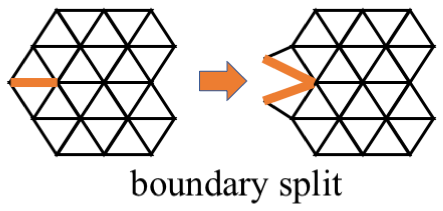
\includegraphics[width=1\linewidth]{fig/bSplit}
  \end{center}
\end{wrapfigure}
When splitting a boundary vertex along an edge connecting to another boundary vertex we either remove a hole or else produce a new chart in our UV map. For the latter case, we generate four duplicate vertices forming the stencil to compute $d$.
%\minchen{[TODO] 4-vertex merge to support joining two charts together, triangle moving operations?}

\paragraph{Interior Vertex Split}
\begin{wrapfigure}[4]{r}{0.4\linewidth}
  \begin{center}
  \vspace{-4mm}
    
\includegraphics[width=1\linewidth]{fig/iSplit}
  \vspace{-1mm}
  \end{center}
\end{wrapfigure}
Interior vertices can be split along 
any pair of incident edges. Each such candidate split generates two duplicate vertices forming the stencil to compute $d$. 
%We ignore potential interior splits when this would be connected to an existing seam, as this is overloaded with propagating the boundary vertex split operation.

\paragraph{Corner Merge}
Corners are formed by three UV vertices corresponding to the tail edge of a cut seam on the input surface. 
\begin{wrapfigure}[5]{r}{0.4\linewidth}
  \begin{center}
  \vspace{-5mm}
    \includegraphics[width=1\linewidth]{fig/cMerge}
  \vspace{-4mm}
  \end{center}
\end{wrapfigure}
Merging the end vertices generates a single new vertex forming the stencil to compute $d$. Merging requires extra care here. Unlike vertex splitting, an initial location for the newly merged vertex must be selected. Na\"ive merging can violate local injectivity and so prevent progress if we are working with barrier-type energies like symmetric Dirichlet. We initialize a merged vertex to the average of its parent vertices. If inversion is detected, we then apply Agmon's relaxation~\shortcite{Agmon1954Relaxation} to iteratively project to an inversion-free position. On rare occasions this will not suffice and so we remove the proposed operation from our queue.
%However, cases are still there when only moving the merged vertex is not enough to obtain an inversion free initial local stencil. In these situations, we will just abandon the candidate. This rarely happens in practice and does not affect our result.\justin{didn't follow the last two sentences, maybe needs a small figure}

\subsection{Topology Search Candidates}
\label{sec:descent_op}
In analogy to computing a continuous search direction, at the start of each new primal solve we search for a candidate mesh operation to propagate descent. 
%
We first consider boundary vertex split originated at one of $m$ boundary vertices in the current topology $T^k$. 
To reduce unnecessary computational overhead we select a subset of $m_\text{test}=m^{0.8}$ boundary vertices that might have the largest effect on the energy. In particular, we compute the standard deviation over all the distortion energy gradients acting on the boundary vertex contributed from incident elements and pick boundary vertices with largest deviation. We use the selected vertices to initiate boundary vertex splits, and consider all available seam tails for a corner merge, building a set of $O^k$ topological operations.
%
%We use the selected vertices to build a set of candidate mesh operations $O^k$ formed by boundary vertex splits and all valid corner merges on those vertices. 
\minchen{The filtering is only applied on split operations, not on corner merge. We simply query all corners, there's not many of them, and the filtering criteria for splits is not appropriate for merge.} 
\vova{how do we know if something is a corner?}
We then find a minimizer
\begin{align}
\label{eq:minO}
o^{i,j} = \argmin_{o \in O^k} d(o).
\end{align}
With local support, all queried $d$ in this minimization can be evaluated in parallel. 

If the minimizing operation promises descent, i.e., $d(o^{i,j}) < 0$, we set our candidate mesh operation for our descent process, $s^k$, with this operation, $s^k \leftarrow o^{i,j}$. Otherwise, we go on to find the $(n-m)^{0.8}$ interior vertices with largest deviation and rebuild $O^k$ as the set of all interior vertex splits on those vertices. A $d$-minimizing interior split operation $o^{i,j} \in O^k$, again using (\ref{eq:minO}), is then set as the set $s^k \leftarrow o^{i,j}$ for our descent process.

\subsection{Iterated Search, Propagation and Descent}
\label{sec:topology_search}
Once we have computed our candidate search operation $s^k$, we begin an inner loop iteration, indexed by superscript $i$ (recalling outer iterates are indexed by $k$), to solve the primal variable update. At the start of this process we initialize our desired upper bound on estimated decrease to $\delta^0 = 0$; this will be updated at each successive iterate. Then, each inner iteration $i$ proceeds by first propagating topology change followed by smooth coordinate update. 

Each topology propagation step first generates a set of all possible mesh operations $\mathcal{E}(s^k, T^{i-1})$ that could continue to propagate the seed operation $s^k$ on topology $T^{i-1}$, e.g. all edges that could continue to propagate a boundary splitting cut from the current tail. See Figure\ \ref{fig:propagation} for illustrations on how we propagate each operation.
As in seeking our seed operation we once again find the $d$-minimizing operation from this small set of candidate operations
\begin{align}
\label{eq:minE}
o^{i,j} = \argmin_{o \in \mathcal{E}(s^k)} d(o).
\end{align}
If this minimizer provides sufficient estimated decrease, so that $d(o^{i,j}) < \delta^{i-1}$, we accept the topology update setting $T^i \leftarrow T^j$; otherwise, we keep topology unchanged with $T^i \leftarrow T^{i-1}.$

\begin{figure}[t]
\centering
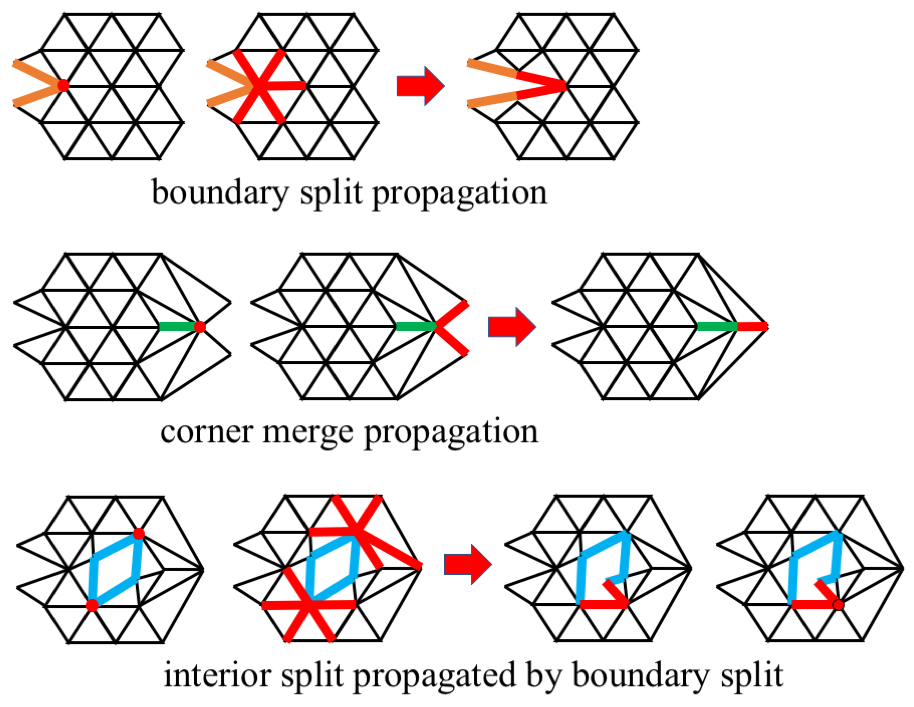
\includegraphics[width=0.8\linewidth]{fig/propagation.png}
\caption{Propagation of boundary split (orange), corner merge (green), and interior split (blue). When propagating boundary split, all edges that could continue to propagate a boundary splitting cut from the current tail would be considered (a); for corner merge we just query the new corner at the current tail (b); for interior split, once an incident edge of either the two tail is splitted as propagation, in the following iterations it would be the same as propagating boundary split (c).
\vova{the rightmost (2nd split result for (c) is confusing. I suggest we remove it} }
\label{fig:propagation}
\end{figure}

The subsequent coordinate update then simply applies a single step of projected Newton descent with line search to update the vertex coordinates $U^i$; see Section~\ref{sec:descentStep} for details. We then ask for the next topology update to gain similar or greater magnitude decrease by setting $\delta^i = E_d(U^i) - E_d(U^{i-1})$.

This process terminates at iteration $i+1$ when smooth iterations have converged (either by gradient or relative error norm) \emph{and} the propagation of the seed mesh operation produces no further descent. We then set $(T^k,U^k) \leftarrow (T^{i+1},U^{i+1})$ and begin the next outer iterate $k+1$ with the dual variable update. 




%\section{Topology Steps for Discrete Optimization}

\subsection{Evaluating Topological Operations via Optimization on Local Stencils}

Candidate Filtering:
for each vertex
  compute divergence of local gradients
independently picking $\sqrt{n_{v,b}^i}$ boundary vertices and $\sqrt{n_{v,i}^i}$ interior vertices with largest divergence as candidates

Local Evaluation:
for each candidate vertex
  if on boundary
    for each interior incident edge
      split and compute $\Delta E_{SD,l}$ locally
      compute $\Delta E_{w,l} = (1 - \lambda_t) \Delta E_{SD,l} + \lambda_t \Delta E_{se}$
  else
    for each pair of incident edges forming a smooth path
      split and compute $\Delta E_{SD,l}$ locally
      compute $\Delta E_{w,l} = 0.5((1 - \lambda_t) \Delta E_{SD,l} + \lambda_t \Delta E_{se})$

split the vertex with largest $|\Delta E_{w,l}|$
turn on fracture propagation

\textcolor{red}{try larger stencils}

\textcolor{red}{enable merge operation}

\textcolor{red}{\subsection{Line Search in Topological Space}}

Current Fracture Propagation:
if fracture propagation is on
  for each fracture tail vertex $k$
    for each interior incident edge of $k$
      split and compute $\Delta E_{SD, l}$ locally
      compute $\Delta E_{w,l} = (1 - \lambda_t) \Delta E_{SD,l} + \lambda_t \Delta E_{se}$
  if the largest $|\Delta E_{w,l}|$ is larger than $|(1-\lambda_t)\Delta E_{SD}^j|$
    propagate fracture by splitting the vertex
  else
    turn off fracture propagation for the rest of the current descent step

% !TeX root = OptCuts.tex

\section{The OptCuts Algorithm}%: Convergence and Implementation Details}
%\section{Implementation Details}
\label{sec:imp}

\begin{algorithm}[t]
\label{alg:OptCuts}
\caption{OptCuts}

\textbf{Given:} $M$, $T^0$, $U^0$, $b_d$ 

\textbf{Initialize:} $\lambda^0 \leftarrow 0$,  \hspace{2pt} \texttt{converged} $\leftarrow$ \textbf{false},  \hspace{2pt} $k \leftarrow 1$\\

\textbf{while} \hspace{2pt} \textbf{!}  \texttt{converged} \hspace{2pt} \textbf{do} \\

%%%----%%%

\hspace{10pt} $\lambda^{k} \leftarrow \max\big(0,\big( E_{d}(T^{k-1}, U^{k-1}) -b_d \big) + \lambda^{k-1}\big)$ \hspace{7pt} // Dual Update (\S\ref{sec:dualUpdate})\\
\hspace{10pt} \texttt{d\_stationary} $\leftarrow$ $| \lambda^{k} - \lambda^{k-1} | < 10^{-3}$ \\

%%%----%%%
\hspace{10pt} // Primal update (\S\ref{sec:primalUpdate}, details in \S\ref{sec:topologySearch}): \\
\hspace{10pt} $i \leftarrow 0$, \hspace{2pt} $(T^{i},U^{i}) \leftarrow (T^{k},U^{k})$, \hspace{2pt} $\delta^{i} \leftarrow 0$ \\
\hspace{10pt} \texttt{v\_converged} $\leftarrow$ \textbf{false}, \texttt{t\_stationary} $\leftarrow$ \textbf{false}, \texttt{t\_stopped} $\leftarrow$ \textbf{false} \\
\hspace{10pt} $o^{0,1} \leftarrow \argmin_{o \in \mathcal{O}^k} d(o)$ \hspace{10pt}//  Get seed topological operation (\S\ref{sec:descent_op})\\

\hspace{10pt} \textbf{if} $d(o^{0,1}) \geq 0$ \\
\hspace{20pt} \texttt{t\_stationary} $\leftarrow$ \textbf{true}\\
\hspace{10pt} \textbf{end if} \\

\hspace{10pt} \textbf{while}  \textbf{!}  ( \texttt{v\_converged} \hspace{2pt} \textbf{and} \hspace{2pt}  \texttt{t\_stopped} ) \hspace{2pt}   \textbf{do} 

%%%----\hspace{20pt} // Topology descent step: \\
\hspace{20pt} \texttt{t\_stopped} $\leftarrow$ \textbf{true} \\
\hspace{20pt} \textbf{if}  \textbf{!} \texttt{t\_stationary} \\
\hspace{30pt} $o^{i,i+1} \leftarrow \argmin_{o \in \mathcal{E}(o^{i-1, i}, T^i)} d(o)$ \hspace{3pt}// Get candidate op (\S\ref{sec:topology_search})  \\
\hspace{30pt} \textbf{if} $d(o^{i,i+1}) < \delta^{i}$ \hspace{10pt} // Sufficient decrease \\
\hspace{40pt} $T^{i+1} \leftarrow o^{i, i+1}(T^i)$ \hspace{10pt} // Update topology (\S\ref{sec:topology_search}) \\
\hspace{40pt} $U^{i+1}_\text{init} \leftarrow (U^{i,i+1}, U_s) $ \hspace{10pt} // Initialize new geometry (\S\ref{sec:topology_search}) \\
\hspace{40pt} \texttt{t\_stopped} $\leftarrow$ \textbf{false} \\
\hspace{30pt} \textbf{else} \\
\hspace{40pt} $T^{i+1} \leftarrow T^i$, \hspace{1pt} $U^{i+1}_\text{init} \leftarrow U^i $ \\
\hspace{30pt} \textbf{end if} \\
\hspace{20pt} \textbf{end if} \\
%%%----\hspace{20pt} // Vertex descent step: \\

\hspace{20pt}  $i \leftarrow i+1$ \\
\hspace{20pt}  $g \leftarrow \nabla_{\small{U}} E_{d}(T^i,U^i_\text{init})$ \hspace{10pt}//  Distortion energy gradient 

\hspace{20pt}\textbf{if} $\|g\| > 10^{-6}$ \hspace{2pt} \\

\hspace{30pt} $H \leftarrow \text{Project}(\nabla_{\small{U}}^2 E_d(T^i,U^{i}_\text{init}))$ \hspace{10pt}// Projected-Hessian (\S\ref{sec:descentStep}) \\

\hspace{30pt} Solve: $H p = -g$ \hspace{10pt} // Get smooth descent direction $p$ (\S\ref{sec:descentStep}) \\

\hspace{30pt} $\alpha \leftarrow \text{LineSearch}(U^{i}_\text{init}, p, E_d)$ \hspace{10pt} // Line-search (\S\ref{sec:descentStep}) \\

\hspace{30pt} $U^{i} \leftarrow U^i_\text{init} + \alpha p$  \\
		
\hspace{30pt} $\delta^{i} \leftarrow E_{d}(T^i,U^{i}) - E_{d}(T^i,U^i_\text{init})$  \\

\hspace{30pt}\textbf{if} $|\delta^{i}/E_{d}(T^i,U^i_\text{init})| < 10^{-6}\alpha$ \textbf{and} \textbf{!}  \texttt{t\_stationary} \\
\hspace{40pt} \textbf{break} \hspace{10pt} // Safe to early exit \\
\hspace{30pt} \textbf{end if} \\

\hspace{20pt} \textbf{else}  \\
\hspace{30pt} \texttt{v\_converged} $\leftarrow $ \textbf{true} \\
\hspace{20pt} \textbf{end if} \\

\hspace{10pt} $\textbf{end while}$ \\

\hspace{10pt}  $(T^{k},U^{k}) \leftarrow (T^{i},U^{i})$ \\

\hspace{10pt} $k \leftarrow k + 1$ \\

\hspace{10pt} \texttt{converged} $\leftarrow$ \texttt{v\_converged} \textbf{and}   \texttt{t\_stationary}  \textbf{and} \texttt{d\_stationary} \\

 $\textbf{end while}$ \\
 
 $(T^{*},U^{*}) \leftarrow (T^{k-1},U^{k-1})$

\end{algorithm}

With the key components now in place, Algorithm 1 summarizes our full OptCuts algorithm in pseudocode, including details on convergence detection and termination. Here, in this section, we next discuss key details including termination/convergence criteria, initialization, preconditioning, and inclusion of global bijectivity constraints.

%details of OptCuts convergence at termination, and 
%then follow with technical details of our implementation of OptCuts. 
%First, we describe our choices for obtaining the initial embeddings. Second, we provide details on continuous search that we use during our smooth descent step. Finally, we provide some details on enforcing and maintaining bijectivity. 

\subsection{Termination and Convergence}
\label{sec:term}

Our primal solution is \emph{converged} whenever it is stationary with respect to variations in both topology \emph{and} vertex position for a fixed $\lambda^k$ multiplier value. Numerically, primal convergence is declared for any $(T^i,U^i)$ pair when 1.) the topology descent is stationary---meaning there are no further available mesh operations at the current multiplier $\lambda^k$ value that will give decrease to the Lagrangian below $L(T^i,U^i,\lambda^k)$;
%at all; 
and 2.) the smooth distortion energy at topology $T^i$ is sufficiently locally minimized so that $\| \nabla_{\small{U}} E_{d}(T^i,U^i)\| \leq 10^{-6}$. When both our primal solve is converged \emph{and} our dual variable is likewise close to stationary so that $| \lambda^k -  \lambda^{k-1}| < 10^{-3}$, OptCuts terminates with a solution that is numerically \emph{converged} to a local minimizer of (\ref{eq:p1}) with respect to all available variations in topology provided by our merge and cut operations. 

%Importantly, our OptCuts algorithm and its implementation \emph{do not} apply a maximum iteration cap anywhere in any of our iteration loops. All presented results and corresponding timings are from solutions that have converged as defined above and in the pseudocode in Algorithm 1. There is, however, one additional, but subtle detail for a robust implementation that warrants further discussion in text rather than in pseudocode---we cover this immediately below.

Importantly, our OptCuts algorithm and its implementation \emph{do not} apply a maximum iteration cap anywhere in any of our iteration loops. All presented results and corresponding timings are from solutions that have converged either as defined above \emph{or} by a cyclic stationarity condition required for a robust implementation that warrants further discussion in text rather than in pseudocode---we cover this immediately below.

First, while we converge with respect to the mesh operations we make available, we of course do not cover all possible topological operations on a mesh. Our choice of propagated cutting and merging operations was selected to cover the basic topology changes that we find suitably expressive for our parameterization task. However, we expect many others to be useful; indeed, below in Section~\ref{sec:var} we also consider and compare with another interesting mesh operation subset and remark that there is interesting future work to find improved mesh operation subsets for OptCuts. In the meantime, for \emph{any} discrete subset of topological operations that do not fully cover all possible mesh changes, \old{there can and will be, a number of neighboring topologies connected by valid mesh operations that are all numerically close to stationarity}\revised{there can and will be discrete sets of points that are stationary with respect to variations of the available mesh operations. In turn, while some of these points will satisfy the imposed distortion bound, they may not match the bound.} In such cases, without additional handling and preparation for cycling behavior, OptCuts would oscillate without stopping between a number of high-quality, close-to-optimal solutions. To handle this condition, we employ a simple cycle detection strategy, where \revised{after each primal solve} we save hashes \revised{$(E_s, E_d, \lambda)$} of \old{previous-iteration} solution triplets, and the best visited solution\old{ from the previous iteration}. When we detect that a duplicate solution is being revisited, we terminate with the best visited solution\old{ from the last iteration}. Of the 254 examples computed with OptCuts in Section~\ref{sec:results}, 171 terminate with cycling about stationarity, while the remainder converge to a stationary point. 
%in 171 and converge to  . As we tighten the distortion bound, cycling behavior decreases as stationary points become denser near isometric maps.

\subsection{Initialization}
%\minchen{to $E_d$ stationary point}% huh?
To initialize our UV map, $(T^0,U^0)$, for an input surface, we map its initial seam to a circle preserving edge lengths and parameterize the remaining vertices with Tutte's embedding~\shortcite{tutte1963draw} using uniform weights to ensure bijectivity.
% Danny: we don't currently do higher genus yet - nothing stopping us but unless we get it in, in time the following needs to go and move to the future work section.
%We compute initial seams for surfaces according to topology and geometry. 
For disk-topology surfaces, we simply pick the longest boundary as an initial seam while for genus-0 closed surfaces, we randomly pick two connected edges as an initial seam. 
% For higher-genus surfaces, we follow Crane et al.~\shortcite{Crane:2013:DGP} to detect homology generators, and connect all of them as an initial seam.
\revised{For higher-genus surfaces we detect homology generators (using the {\tt cut\_to\_disk} function in libigl\ \cite{libigl}) and then connect them to form an initial seam.}
%%
We then set $(T^0,U^0)$ to this initial topology with vertex positions minimizing distortion, $E_d$, on the initial embedding, and start OptCuts by initializing $\lambda^0 = 0$. This sets the first iteration to initially ignore distortion and so begin by exploring a shortening of seam lengths.% first.


%From the initial UV map, we simply start the optimization by ignoring the distortion constraints with $\lambda$ set to $0$ and let our dual update to modify $\lambda$ according to the distortion of intermediate results.

%\danny{Minchen: are we likely to do this next experiment in time? I think it's low priority -- we may just want to get rid of this next section?}
%For closed surfaces, the initial seam choice is one of many possibilities. To demonstrate insensitivity of our final embedding to this choice, %show that we can always find a local optimum with respect to both the UV topology and coordinates regardless of initial embedding, 
%we run our method on a closed input surface with several randomly picked initial seams, as well as a heuristic initial seam that splits the shortest path between two farthest points on the surface. As demonstrated in \minchen{Figure~\ref{fig:any_init_ends_well}}, we produce high quality UV maps under the given distortion bound for all initializations.

\subsection{Minimizing Distortion}
\label{sec:descentStep}

Each smooth descent step takes as input a possibly updated UV map from the previous topology descent step and applies a single Newton-type iteration to reduce $E_d$ over changes in vertex positions $U$ while holding topology, $T$, fixed.
%
%\begin{algorithm}[h]
%\SetAlgoLined
%\KwData{$M$, $T^{k,i}$, $U_a^{k,i-1}$}
%\KwResult{$U^{k,i}$, $\delta^{k,i}$}
%$g^{k,i-1} \leftarrow \nabla E_{d}(T^{k,i}, U_a^{k,i-1})$\;
%\If{$||g^{k,i-1}||^2 < 10^{-12}$}{
%	converge\;
%}
%compute $E_{d}$ Hessian proxy $P^{k,i-1}$\;
%solve $P^{k,i-1} p^{k,i-1} = -g^{k,i-1}$ for search direction $p^{k,i-1}$\;
%compute initial step size $\alpha^{k,i-1}_0$\;
%back-tracking line search with Armijo rule to obtain $\alpha^{k,i-1}$\;
%$U^{k,i} \leftarrow U_a^{k,i-1} + \alpha^{k,i-1} p^{k,i-1}$\;
%$\delta^{k,i} \leftarrow E_{d}(T^{k,i}, U^{k,i}) - E_{d}(T^{k,i}, U_a^{k,i-1})$\;
%\If{$|\delta^{k,i}/E_{d}(T^{k,i}, U_a^{k,i-1})| < 10^{-6}\alpha^{k,i-1}$}{
%	stop\;
%}
%\caption{Smooth Descent Step $(k+1,i)$}
%\label{alg:descentStep}
%\end{algorithm}
As our distortion energies $E_{d}$ are generally nonconvex, we apply Teran et al.'s\ \shortcite{Teran2005Robust} projected-Newton (PN) method to gain a modified Hessian proxy that is guaranteed PSD. We parallelized PN's per-element Hessian construction,   projection and assembly into the PN Hessian proxy, $H$, with Intel TBB~\cite{Reinders2007Intel}.  We then apply Pardiso~\cite{pardiso-6.0a, pardiso-6.0b} to solve the resulting linear system for the next descent direction. For line search we first use Smith and Schaefer's~\shortcite{Smith2015Bijective} line-search filter to avoid element inversion followed by standard line search with Armijo conditions~\shortcite{Armijo1966Minimization} to ensure sufficient energy decrease. Finally, we employ one additional optimization that is specific to OptCuts: on smooth steps where we are \emph{not} yet stationary with respect to topology operations, there is no need to expend extra iterations to gain tight convergence on distortion. In these cases we terminate iterations when we simply have the more relaxed condition of small change in energy. On the other hand, when a stationary topology is reached, we then always require and apply full convergence to small gradient norm of $E_d$; see Algorithm 1.
%$ H p = - \nabla E_d(U)$ to gain descent direction $p$.

%to project the Hessian of each energy element to its closest symmetric positive definite (SPD) matrix in parallel with Intel TBB~\cite{Reinders2007Intel} and assemble the local Hessians to form an SPD Hessian proxy $P$ for the full mesh. We use the PARDISO~\cite{pardiso-6.0a, pardiso-6.0b} symmetric indefinite solver to solve the linear system $P p = -g$ for search direction $p$. \minchen{[TODO] change to use SPD solver by fixing a direction to ensure definiteness} As $E_{d}$ is also a barrier-type energy, it is essential to ensure that the configuration always stays inside the feasible region. Thus, we follow Smith and Schaefer~\shortcite{Smith2015Bijective} to compute an initial step size $\alpha_0$ that avoids element inversion and then conduct back-tracking line search with Armijo rule~\cite{Armijo1966Minimization} to ensure sufficient energy decrease.
%
%Besides a relatively small tolerance on $g$ for convergence detection, we apply another relative energy decrease criteria to appropriately stop the process while necessary.
%This can stop our continuous search at the true local optimum infinitesimal better than setting a larger gradient tolerance since our energy is highly nonlinear. \justin{I didn't follow this paragraph.}

\subsection{Global Bijectivity}
\label{sec:bijectivity}

Following Jiang et al.\ \shortcite{Jiang2017Simplicial}, we apply global bijectivity constraints to our mapping by (re-)triangulating void regions each time we update our UV map. We use the Triangle library~\cite{shewchuk1996triangle}. Void regions consist of all holes as well as a loose bounding box enclosing the UV map.
We then add to our distortion energy $E_d$ an additional term \emph{not included in the distortion bound constraint} on these void triangles to form a collapse-preventing energy for the added negative-space triangles during each primal optimization iteration.

Our continuous descent steps on vertices then remains otherwise unchanged.
However, for each topology step, we need to ensure that negative-space triangles are inserted correctly for each query of a candidate local topological operation. Here, there are two simple modifications we need to apply. First, for local queries of descent per candidate query minimizations evaluating $d$, we need only triangulate the void region about the union of one rings around the participating stencil vertices. This provides a sufficient scaffold to ensure bijectivity in the local solve without growing the problem size. Second, for each candidate edge split we need to carefully pull apart the new split vertices to form an initial void to build the scaffold triangulation. We pull the duplicated vertices along their curvature normals far enough to form a gap while ensuring no triangle elements are inverted. 

%\danny{Minchen: ping me to discuss these next 2 paragraphs - not sure it's consistent with what I thought you were doing.}
%Instead of reusing a loose bounding box, we take the current negative-space triangles into consideration when building up the local stencil near the edited seam. Since the boundary of the local stencils are all fixed during the query, this naturally prevents potential global overlaps with geodesically faraway UV elements. Similarly, the collapse preventing energy on the negative-space triangles is not involved in the computation of first-order reduction.
%
%In splitting operations only, we also need to carefully push the split vertices in the opposite direction of their curvature normals before the querying optimization. This ensures that the initial local stencil has a collapse-free void region so that it could be triangulated correctly. 


%Following Jiang et al.\ \shortcite{Jiang2017Simplicial}, we realize the global bijectivity constraint on our mapping by first triangulating the void regions of each iterations updated UV map using Triangle library~\cite{shewchuk1996triangle}. The void regions consist of all holes and the surrounding space of the UV map, bounded by the parameterization's boundaries and a loose bounding box.
%We augment our distortion energy $E_d$ with an additional term \emph{not included in the distortion bound constraint} to form a collapse-preventing energy for the added negative-space triangles during each optimization iteration.
%
%With this augmentation, our continuous search stays the same, while for our topology search, we need to also ensure that the negative-space triangles are added correctly when we query for our local topological operations.
%Instead of reusing a loose bounding box, we take the current negative-space triangles into consideration when building up the local stencil near the edited seam. Since the boundary of the local stencils are all fixed during the query, this naturally prevents potential global overlaps with geodesically faraway UV elements. Similarly, the collapse preventing energy on the negative-space triangles is not involved in the computation of first-order reduction.
%In splitting operations only, we also need to carefully push the split vertices in the opposite direction of their curvature normals before the querying optimization. This ensures that the initial local stencil has a collapse-free void region so that it could be triangulated correctly.

%\paragraph{Potential Accelerations for Practical Use}
%Since our topological operations only change the mesh locally both on connectivity and coordinates, we could also update the Hessian or the decomposition locally to save time. Besides, it is also interesting to try other Hessian approximation methods like L-BFGS~\cite{Liu1989Limited} or composite majorization~\cite{Shtengel2017Geometric} to explore further acceleration by finding a balance between per-iteration computational cost and convergence rate.
%\justin{not sure previous paragraph is needed}




% !TeX root = OptCuts.tex

\section{Results and Discussion}
\label{sec:results}

\subsection{Experiments}

\paragraph{Initial Embedding} For disk-topology surfaces, we map the longest boundary to a circle preserving edge length and obtain a Tutte embedding with uniform weights \minchen{[TODO] see whether using MVC weights converge faster}. For closed surfaces (including high-genus surfaces), we first apply some simple heuristics to obtain an initial seam, and then treat them as disk-topology surfaces. 
The heuristics for genus-0 surfaces include farthest point cut and random/curvest one point cut \minchen{[TODO] decide one and add description, or use all?}; for high-genus surfaces, we follow Crane et al.~\shortcite{Crane:2013:DGP} to detect homology generators and then cut along all of them \minchen{[TODO]}.
In order to show that we search for locally optimal UV maps regardless of the given initial embedding, we run our method starting from triangle soup and preliminary UV maps produced by other methods or by the users. The output maps are still with high quality (Figure~\ref{fig:bad_init_still_ends_well}) \minchen{[TODO]}.

\paragraph{Quality and Timing Comparisons} \minchen{[TODO], also provide detailed settings on the compared methods, and how much user assistance was needed for other methods?} We demonstrate our framework's capabilities by first comparing to AutoCuts~\cite{Poranne2017Autocuts} and two typical classic seam cutting methods~\cite{Gu2002Geometry,Sheffer2002Seamster}. Given the same input surface and initial UV map, we efficiently reach identical distortion bounds with shorter seam lengths (Figure~\ref{fig:QT_comp}). 
When we change the settings in order to obtain nearly isometric UV maps, the quality of the seams by other methods drop drastically while our method keeps generating high-quality seams (Figure~\ref{fig:strict_bounds_comp}).

\paragraph{Triangulation Invariance} \minchen{[TODO] not sure whether applicable}

\paragraph{Scalability Test} \minchen{[TODO]}

\subsection{Variations}

Without changing the framework, simply reformulating $E_w = E_s + \lambda E_d$ according to different needs enables OptCuts to solve mesh parameterization problems in many variations:

\paragraph{Global Bijectivity} \minchen{[DOING]} Augmenting our $E_s$ with a collision handling energy $E_b$ will easily achieve joint seam placement and bijective mesh parameterization. We show that by adding a scaffold mesh~\cite{Jiang2017Simplicial} to the voided regions of the UV map and preventing the scaffold mesh from degenerate, our method automatically generate high-quality bijective maps with optimal seams different from that of locally injective parameterization (Figure~\ref{fig:bijective_vs_injective}).

\paragraph{Conformal Parameterization} \minchen{[TODO]} Using a conformal energy~\cite{Hormann2000MIPS,Sheffer2005ABFPP} for $E_s$ will achieve joint seam placement and conformal parameterization. Figure~\ref{fig:conformal_vs_isometry} shows some results with $E_s = E_{ABForMIPS}$~\cite{} compared to results with $E_s = E_{SD}$, where different seams are generated while our framework stays the same.

\paragraph{Regional Seam Placement} \minchen{[TODO]} On the discrete side, if we reweight $E_{SL}$ with an edge prior provided by the user or an algorithm~\cite{} as
\[ E_s = \hat{E}_{SL} = \sum_{i\in\mathcal{S}} w_{SL,i} E_{SL,i} \quad w_{SL,i} \in \mathcal{R^+} \]
we could bias the seam placement towards regions e.g. where continuity is less in demand (Figure~\ref{fig:regional_seam_placement}).

discoveries? like interior splits?

\section{Conclusions and Future Works}

\begin{itemize}
\item Our method doesn't provide globally optimal solutions, the results are still locally optimal, but w.r.t. both seams and distortion, which is better than previous 2-pass methods that breaks the correlation between seams and distortion.
\item take advantage of basic SIMD type of parallelism for accelerating query and improving results' quality by directly evaluating $f_v$ for neighbors and track multiple branches, very useful for practical implementations
\item if the user won't mind getting a slightly different triangulation, we could also create fractures in the interior of an element and locally remesh the stencil
\item start and solve in 3D by reducing curvature so that the need for locally injective initial embedding in parameterization problems could be eliminated, and the result is only "biased" by it's 3D shape, which is the most reasonable bias
\item try conformal energy like MIPS
\item \textcolor{red}{bijectivity}, seamless, and other augmentation of continuous energy?
\item handle user preferences on seam placement
\item seam smoothness, patch related discrete energy augmentation?
\end{itemize}

\section{Acknowledgements}

\bibliographystyle{ACM-Reference-Format}
\bibliography{OptCuts} 

\appendix

\section{Auto-mode AutoCuts}
\label{app:autoauto}

Recall that in the AutoCuts model the topology of the UV mesh does not change: it remains a triangle soup. Instead, the seam-penalty energy that pulls triangles together is parameterized by a $\delta$ parameter which indicates how far vertices must be from one another to be considered truly disconnected by a seam. Finding a single weighting $\lambda$ that works well for all geometries poses a challenge and likewise $\delta$ requires adjustment over iterations depending on the current stage of the optimization. Thus AutoCuts is generally most effective in interactive mode with a user in-the-loop. For instance, starting from a disconnected triangle soup, a user will gradually decrease $\delta$ defining a {\em homotopy path} over the course of optimization to arrive at a final set of seams. The user also needs to move parameterized components to guide the UV layout towards a globally bijective solution. 

Here the key step in formulating the automated mode for AutoCuts is in automating the homotopy path. This requires prescribing an automated sequence of updates to $\delta$ with a uniform set of mesh-adaptive parameters. In final we set the Autocut parameter $\lambda = 0.4$ and start with $\delta_0=100\xi^2$. We then half this value at the start of each homotopy iteration $\delta_i = \frac{1}{2}\delta_{i-1}$ until it reaches $\delta_\text{term}=10^{-4}\xi^2$. Inside each homotopy iteration, we detect convergence by setting a tolerance $\sqrt{3n_t}\times10^{-3}\xi$ on the $L^2$ norm of UV coordinate changes. Here $\xi$ is the characteristic value of the average edge length in the mesh while $n_t$ is the number of triangles---we seek to make these automated measures robust over varying mesh-resolutions as well as scale.

\end{document}
